%
% File coling2020.tex
%
% Contact: feiliu@cs.ucf.edu & liang.huang.sh@gmail.com
%% Based on the style files for COLING-2018, which were, in turn,
%% Based on the style files for COLING-2016, which were, in turn,
%% Based on the style files for COLING-2014, which were, in turn,
%% Based on the style files for ACL-2014, which were, in turn,
%% Based on the style files for ACL-2013, which were, in turn,
%% Based on the style files for ACL-2012, which were, in turn,
%% based on the style files for ACL-2011, which were, in turn, 
%% based on the style files for ACL-2010, which were, in turn, 
%% based on the style files for ACL-IJCNLP-2009, which were, in turn,
%% based on the style files for EACL-2009 and IJCNLP-2008...

%% Based on the style files for EACL 2006 by 
%%e.agirre@ehu.es or Sergi.Balari@uab.es
%% and that of ACL 08 by Joakim Nivre and Noah Smith

\documentclass[11pt]{article}
\usepackage{coling2020}

\usepackage{CJKutf8}
\def\yin#1{\begin{CJK*}{UTF8}{gbsn}#1\end{CJK*}}


\usepackage{times}
\usepackage{url}
\usepackage{latexsym}
\renewcommand{\UrlFont}{\ttfamily\small}
\usepackage{float}
% This is not strictly necessary, and may be commented out,
% but it will improve the layout of the manuscript,
% and will typically save some space.
\usepackage{microtype}
%\usepackage[UTF8]{ctex}
\usepackage{graphicx} 
\usepackage{float} 
\usepackage{subfigure} 
\usepackage{graphicx}
\usepackage{subfigure}
%\usepackage{subcaption,booktabs}
%\usepackage{wrapfig}
%\aclfinalcopy % Uncomment this line for the final submission
%\def\aclpaperid{***} %  Enter the acl Paper ID here

%\setlength\titlebox{5cm}
% You can expand the titlebox if you need extra space
% to show all the authors. Please do not make the titlebox
% smaller than 5cm (the original size); we will check this
% in the camera-ready version and ask you to change it back.

% START custom header
\usepackage{amsfonts}
\usepackage{bm}
\usepackage{array,amsmath}
\usepackage{amssymb}
\usepackage{dsfont}
\usepackage{float}
\usepackage{graphicx}
\usepackage{algorithm}
\usepackage{algorithmicx}
\usepackage{algpseudocode}
\usepackage{pgf,tikz}
\usepackage{mathrsfs}
\usepackage{multirow}
\usepackage{booktabs}
\usetikzlibrary{arrows}
\usepackage{threeparttable}

\def\figref#1{Figure~\ref{fig:#1}}
\def\figlabel#1{\label{fig:#1}\label{p:#1}}
\def\chapref#1{Chapter~\ref{chap:#1}}
\def\chaplabel#1{\label{chap:#1}\label{p:#1}}
\def\Tabref#1{Table~\ref{tab:#1}}
\def\tabref#1{Table~\ref{tab:#1}}
\def\tablabel#1{\label{tab:#1}\label{p:#1}}
\def\Secref#1{\S\ref{sec:#1}}
\def\secref#1{\S\ref{sec:#1}}
\def\seclabel#1{\label{sec:#1}}
\def\eqref#1{Eq.~\ref{eqn:#1}}
\def\eqrefn#1{\ref{eqn:#1}}
\def\eqsref#1#2{Eqs.~\ref{eqn:#1}/\ref{eqn:#2}}
\def\eqlabel#1{\label{eqn:#1}}
\def\subsp#1{P_{\mbox{{\scriptsize\rm #1}}}}

\def\numpar{100k}
\def\ppnumpar{5}

\newcounter{notecounter}
\newcommand{\enotesoff}{\long\gdef\enote##1##2{}}
\newcommand{\enoteson}{\long\gdef\enote##1##2{{
			\stepcounter{notecounter}
			{\large\bf
				\hspace{1cm}\arabic{notecounter} $<<<$ ##1: ##2
				$>>>$\hspace{1cm}}}}}
\enoteson
%\enotesoff
\long\def\eat#1{}

\def\dnrmupmath#1#2{\mbox{$^#2_{\hbox{\scriptsize #1}}$}}
\def\dnrm#1{\mbox{$_{\hbox{\scriptsize #1}}$}}
\def\uprm#1{\mbox{$^{\hbox{\scriptsize #1}}$}}
\def\cupequal{\cup\!\!=}
\newcommand{\pluseq}{\mathrel{+}=}


%\setlength\titlebox{5cm}
%\colingfinalcopy % Uncomment this line for the final submission

% You can expand the titlebox if you need extra space
% to show all the authors. Please do not make the titlebox
% smaller than 5cm (the original size); we will check this
% in the camera-ready version and ask you to change it back.


\title{Monolingual and Multilingual Reduction of Gender Bias in Contextualized Representations}

\author{First Author \\
  Affiliation / Address line 1 \\
  Affiliation / Address line 2 \\
  Affiliation / Address line 3 \\
  {\tt email@domain} \\\And
  Second Author \\
  Affiliation / Address line 1 \\
  Affiliation / Address line 2 \\
  Affiliation / Address line 3 \\
  {\tt email@domain} \\}

\date{}

\begin{document}
\maketitle
\begin{abstract}
	
Pretrained language models (PLMs) learn stereotypes held by
humans and reflected in text from their training corpora,
including gender bias.  When PLMs are used for downstream
tasks such as picking candidates for a job, people's lives
can be negatively affected by these learned stereotypes.
Prior work usually identifies a linear gender subspace and
removes gender information by eliminating the
subspace. Following this line of work, we propose to use DensRay, an
analytical method for obtaining interpretable ultradense
subspaces. We show that DensRay performs on-par with prior
approaches, but provide arguments that it is more robust. By applying DensRay to attention heads and layers to BERT 
we show that gender information is spread across all attention heads and most of the layers.  Finally,
we demonstrate that we can remove bias multilingually, e.g.,
from Chinese, using only English training data.
	
\end{abstract}


\section{Introduction}
Word embeddings, which represent the semantic meaning of
text data as vectors, are used as input in natural language
processing tasks. It has been found that word embeddings
exhibit biases such as gender bias, which are present in their training
corpora \cite{bolukbasi2016man,caliskan2017semantics,garg2018word}. Contextual word
embedding models, such as BERT \cite{devlin2018bert}, have
become increasingly common and achieved new state-of-the-art
results in many NLP tasks. Researchers have also found
gender bias in contextualized
embeddings ~\cite{zhao2019gender,may2019measuring}.

A common approach for removing gender information in static
embeddings is to identify a linear gender subspace (e.g., a
gender direction) and subsequently setting all values on the
gender direction to 0. Successful approaches rely on simple
principal component
analysis \cite{bolukbasi2016man,mu2018all}. \newcite{bolukbasi2016man}
require pairs of gendered words to compute a direction
(e.g., ``man''-``woman'') and \newcite{mu2018all} rely on
computing a PCA of a set of gender words hoping that the
main variation occurs across gender. We propose to use
DensRay \cite{dufter2019analytical}: the main advantage is
that DensRay only requires two or multiple groups of
gendered words. In contrast to \cite{bolukbasi2016man}, it
does not require explicit pairs. Compared
to \cite{mu2018all}, it has explicit supervision with gender
labels. We show in \secref{artexample} that this is leads to better gender directions identified by 
DensRay.

In summary, our contributions are: 
i) We adjust DensRay to be usable to debias contextualized embeddings
By evaluating the approach on two tasks, a set of templates we constructed and previously used Association Tests, we show that DensRay performs comparable to prior approaches. 
ii) We provide arguments why DensRay is more robust and find that applying DensRay affects language model performance on downstream tasks less.
iii) We analyse how gender information is processed in BERT by applying DensRay to attention heads and layers: we conclude that there is no single attention head responsible for processing gender information. In addition we show in a qualitative analysis that token-level gender scores can be obtained. 
v) We apply our debiasing method to the multilingual-BERT (mBERT) model: we show that English training data can be used to effectively debias Chinese.



\section{Methodology}
\subsection{Debiasing Conceptor}
In this paper, we will compare our work with the debiasing conceptor \cite{karve2019conceptor}. Given a set of gendered words $V:=\{v_1,v_2,\dots,v_n\}$ and their embeddings $E \in R^{n\times d}$, gender bias can be mitigated by multiplying the debiasing conceptor matrix$\neg C= I-C$, where $C$ is the conceptor matrix that minimizes the objective
\begin{eqnarray}
||E-CE||^2_F+\alpha^{-2}||E||^2_F
\end{eqnarray}
where $\alpha$ is a parameter. $C$ has an analytical solution
\begin{eqnarray}
C=\frac{1}{n}EE^T(\frac{1}{n}EE^T+\alpha^{-2}I)^{-1}
\end{eqnarray}
Intuitively, C is a soft projection matrix on the linear subspace where the word embeddings have the maximum bias.

\subsection{Hard Debasing}
We will also compare with the hard debiasing method proposed
by \newcite{mu2018all}, which is originally a postprocessing
technique for improving word
representations. \newcite{karve2019conceptor} adopted it as a
method for debiasing. Hard debiasing relies upon
the assumption that the first principal component of the
embedding vectors is a meaningful gender direction. 
PCA is used to obtain the first
principal component from the embeddings of gendered words
and to project it off.

\subsection{DensRay}
DensRay is an analytical method for identifying the
embedding subspace of certain linguistic features. We aim to
identify the ``gender subspace'' using a set of gendered words
$V:=\{v_1,v_2,\dots,v_n\}$ and their embeddings $E \in
R^{n\times d}$, thus for word $v_i$ we have the
corresponding embedding vector $e_{v_i}$. We
introduce a function $l$ for the gender attribute:
$l:V\to \{-1,1\}$;
e.g. $l(\mbox{father})=1$, $l(\mbox{sister})=-1$. The objective of DensRay
is to find an orthogonal matrix $Q\in R^{d\times d}$ such
that $EQ$ is gender-interpretable, specifically, the first
$k$ dimensions can be interpreted as the gender subspace.

Let $L_{=}:=\{(v,w)\in V\times V|l(v)=l(w)\}$ and define
$L_{\neq}$ analogously.  The DensRay objective
in \eqref{densray1} is to maximize the distance of the word
pairs from the same gender group ($L_{=}$) and minimize the
distance of the word pairs from the different gender group
($L_{\neq}$).
\begin{eqnarray}
\max\limits_{q} 
\sum_{(v,w)\in L_{\neq}}\alpha_{\neq}||q^Td_{vw}||^2_2
-\sum_{(v,w)\in L_{=}}\alpha_{=}||q^Td_{vw}||^2_2
\eqlabel{densray1}
\end{eqnarray}
where we define $d_{vw}:=e_v-e_w$. We also have $q\in R^d$
and $q^Tq=1$ since $Q$ is orthogonal. $\alpha_{\neq},\alpha_{=}\in [0,1]$ are hyperparameters. Observing that $||x||^2_2=x^Tx$, objective \eqref{densray1} can be simplified to:
\begin{eqnarray}
\max \limits_{q} q^T(
\sum_{(v,w)\in L_{\neq}}\alpha_{\neq}||d_{vw}d_{vw}^T||^2_2-\sum_{(v,w)\in L_{=}}\alpha_{=}||d_{vw}d_{vw}^T||^2_2)q=:\max\limits_{q} q^TAq
\eqlabel{eq:densray2}
\end{eqnarray}

This objective is maximizing the Rayleigh quotient of $A$ and $q$. Since $A$ is symmetric, we can get an analytical solution $q$ by the eigenvector with the max eigenvalue of $A$ \cite{horn1990matrix}. Thus the matrix of $k$ eigenvectors of $A$ ordered by the corresponding eigenvalues yields the matrix $Q$.
\subsection{Removing Gender Information}

All prior methods yield a gender dimension $q \in R^d$. In a contextualized language model like BERT each layer yields a contextualized embedding matrix $X \in R^{t \times d}$ where $t$ is the length of the sentence. To debias representations we simply zero out the projected values on $q$ for each position, that is we set $X^{\text{debiased}}_i = X_i -  (X_i^\intercal q) q$ for each position $i$.

\seclabel{artexample}
 \figref{fig:example} shows artificially created two dimensional embeddings. The lines show the gender directions identified by hard debiasing, debiasing conceptor, and DensRay. 
 
 DensRay separates the gendered words into two gender groups to produce a meaningful gender direction by objective \eqref{eq:densray2}, while debiasing conceptor and hard debiasing compute the subspace with the whole gendered words set. Theoretically, they may fail to identify the correct gender direction in some cases. 
\begin{figure}[h]
	\centering
	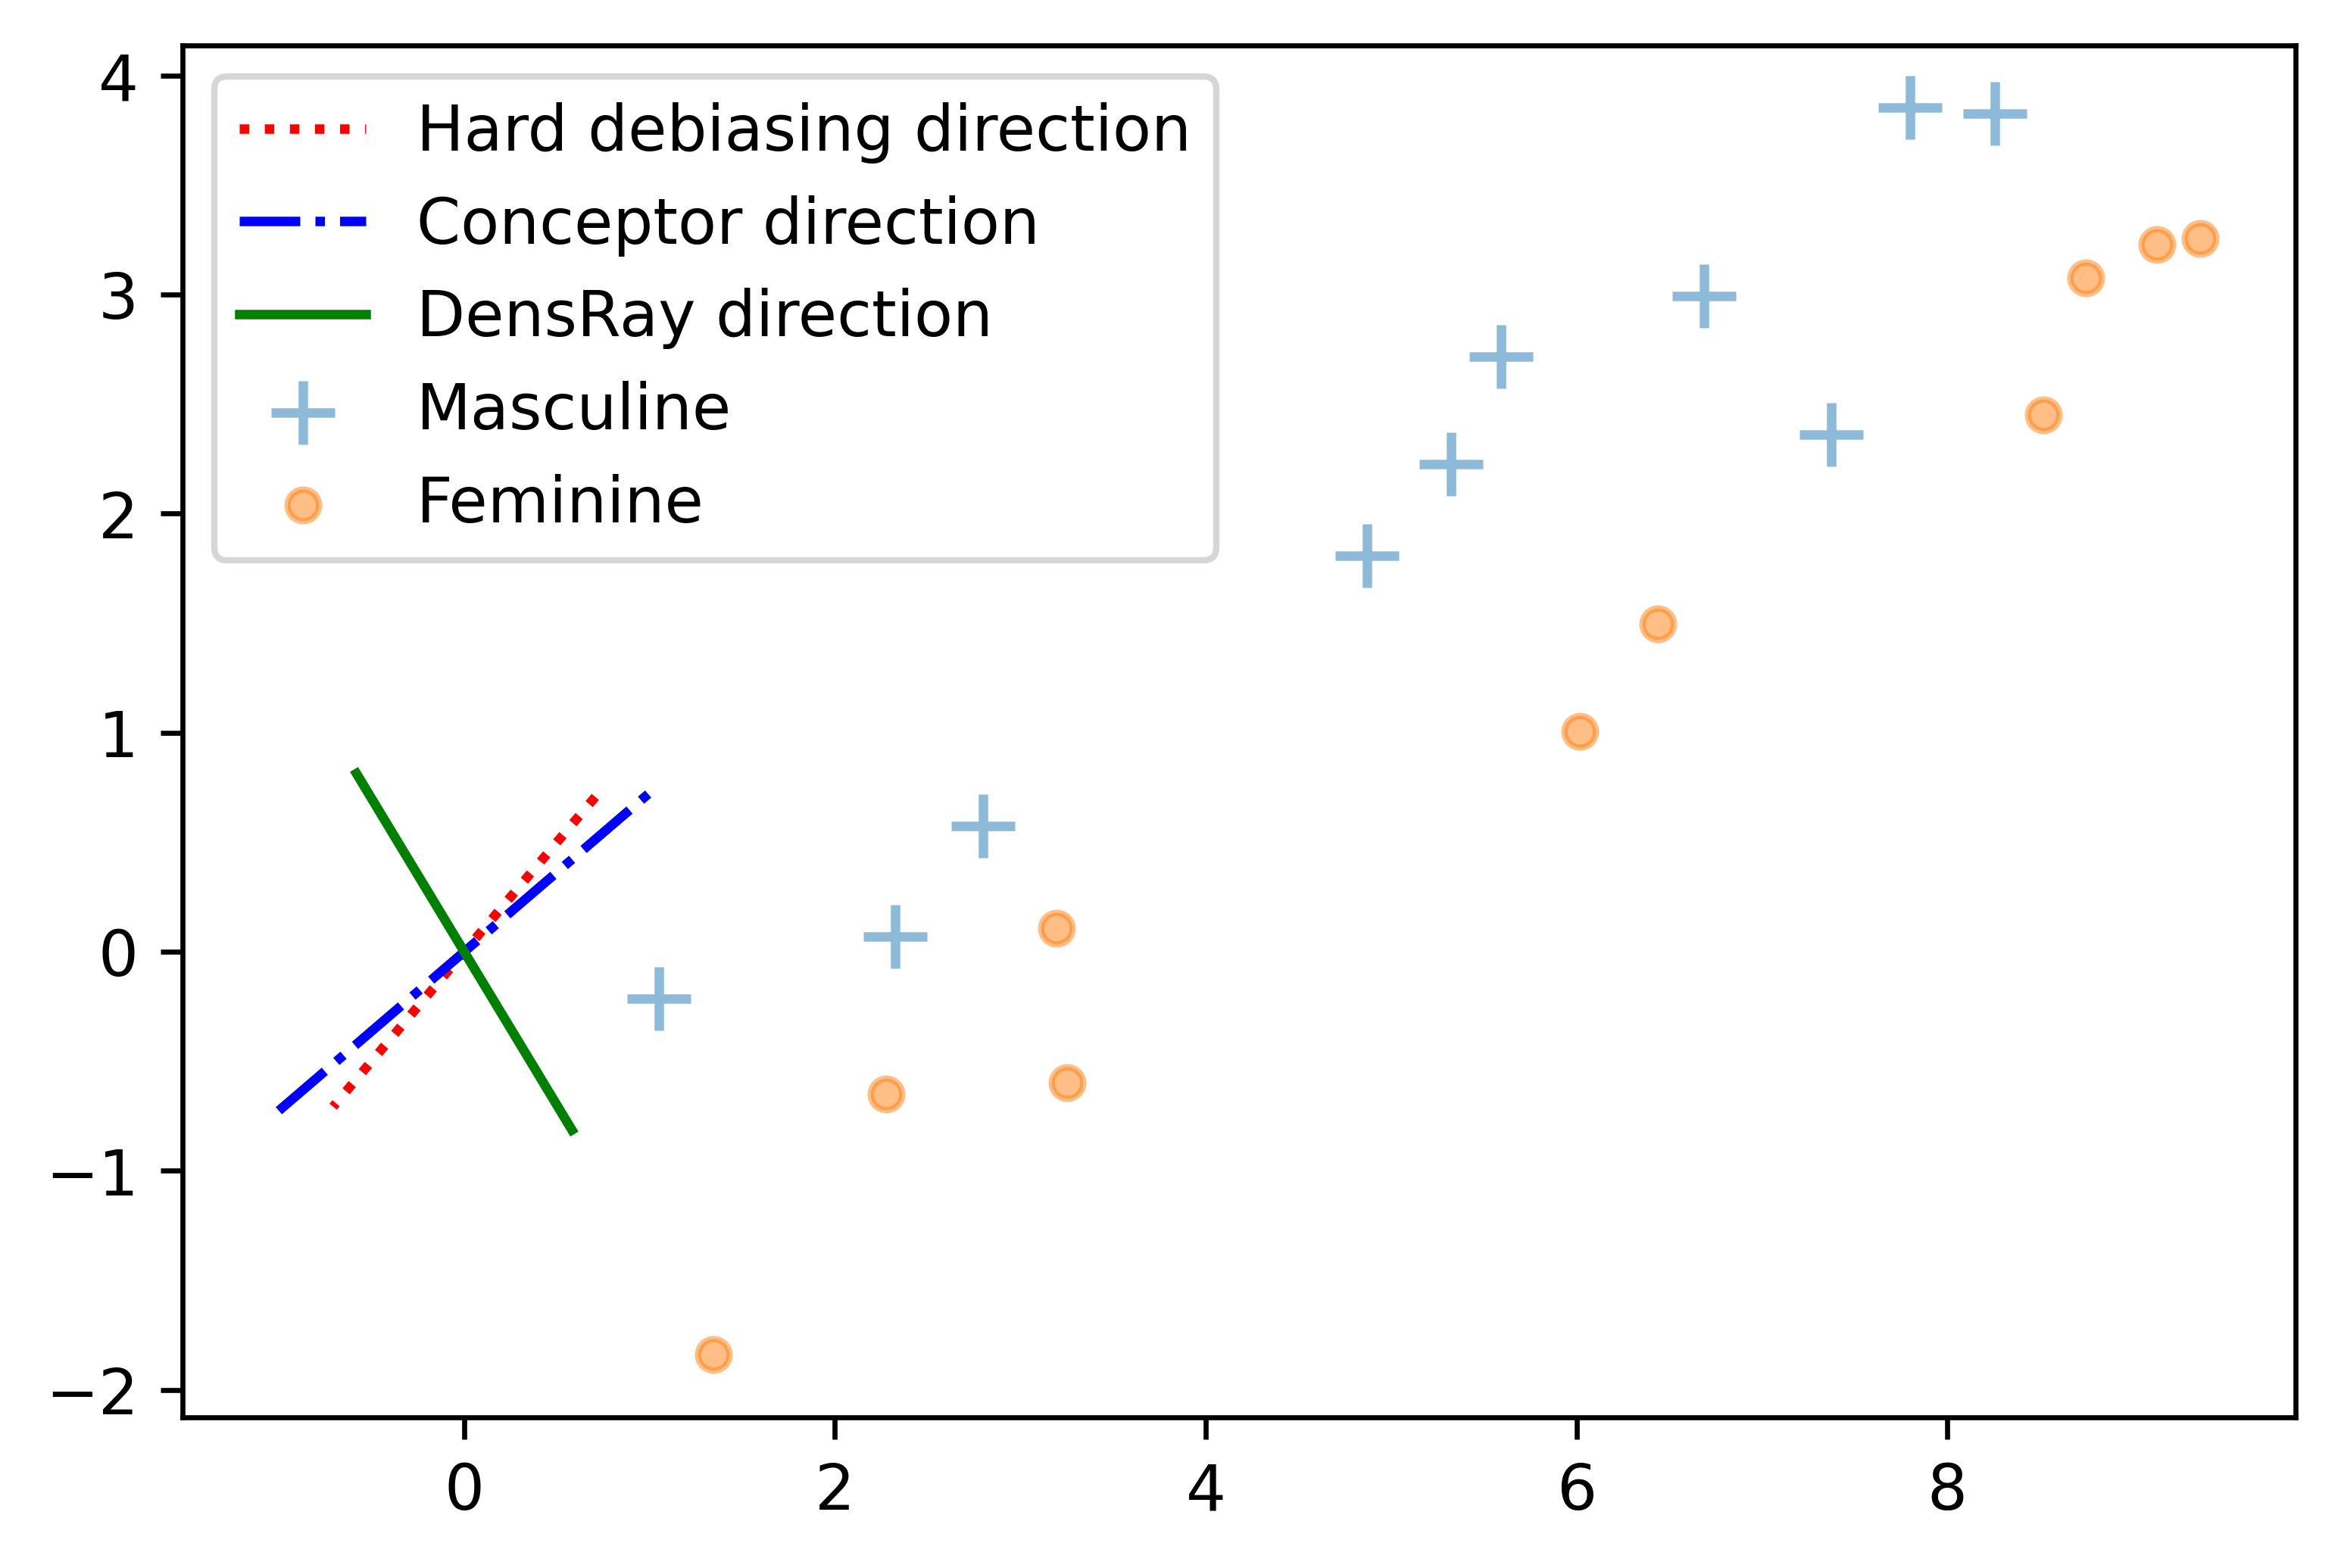
\includegraphics[width=0.5\linewidth]{examples.png}
	\caption{Gender direction on gendered words.}
	\figlabel{fig:example}
\end{figure}

\subsection{Adapting DensRay to Contextualized Language Models}
We now describe how we adapt DensRay to contextualized
language models. Given a set of gendered words
$V$, we extract sentences containing a word in $V$ from a
corpus. We run a contextualized language model
with $M$ layers
on each
sentence
$t_1,\ldots,t_j,\ldots,t_n$ (where $t_j \in V$)
and compute the contextualized representations $e^m, 1\leq m
\leq M$ of $t_j$, one for each layer. 
We compute an orthogonal rotation
matrix $Q_m$ for the $m$th BERT layer using \eqref{eq:densray2}.
For debiasing, we set the gender subspace dimensions to $0$ to eliminate or at least reduce gender information that may cause bias. In this paper, we take the first dimension of the rotated space as the gender subspace.



\section{Experiments}
\subsection{Experiments Setup}
In the experiments we use the BERT models "bert-base-uncased" and "bert-large-uncased". We implemented all experiments using the transformers library \citep{wolf2019huggingfaces}.

To compute the rotation matrices by DensRay, we need a gendered word list as label, and some corpus. For the word list, we get 23 masculine words and 23 feminine words from the "family" category\footnote{http://download.tensorflow.org/data/questions-words.txt} of the Google analogy test set \citep{mikolov2013efficient}, and label them as 1 and -1. As the input corpus, we collect text data from Wikipedia that contains 5,000 (10,000) occurrences of words in the gendered list. We carefully balance the occurrences such that the number of male and female samples are equal. We set  $\alpha_{\neq}=\alpha_{=}=0.5$, as we have balanced the training samples from the corpus.

\subsection{Results on Templates}
Results about our experiments on the templates are summarized in table \ref{t:templates1}. Two example templates are given in table \ref{t:templates2}. The evaluation on our templates shows that DensRay can mitigate the gender bias on BERT: the average difference between predicting he/she drops by more than half (e.g., bert-base from 0.47 to 0.17)
\begin{table*}[ht]
\centering
\footnotesize
\begin{tabular}{lllll}
\hline
model & prob(he) & prob(she) & diff & var\\
\hline
bert-base & 0.6594 & 0.1874 & 0.4720 & 0.1600 \\
bert-base-densray & 0.5106 & 0.3447 & {0.1658} & 0.0119\\
\hline
bert-large  & 0.6287 & 0.1907 & 0.4380 & 0.1262 \\
bert-large-densray  & 0.4751 & 0.2923 & {0.1827} & 0.0150\\
\hline
\end{tabular}
\caption{ \enote{pd}{I think two digits are sufficient here instead of 4?} \enote{pd}{would be great to use figlabel and figref, or tablabel and tabref}\label{t:templates1}
BERT debiasing results on templates. \textit{bert-base} and \textit{bert-large} are the original model without debiasing. \textit{prob(he)} is the mean probability that model predict \textit{he} as the [MASK]in all templates. \textit{var} is the variance of the differences between the probability of BERT predicts [MASK] as \textit{he} and \textit{she}.}
\end{table*}
\begin{table*}[ht]
\centering
\footnotesize
\begin{tabular}{llll}
\hline
sentence & model & prob(he) & prob(she)\\
\hline
[MASK] is a adjunct professor. & bert-base & 0.7231 & 0.1942\\
 & bert-base-densray & 0.4423 & 0.4740\\
 & bert-large & 0.7181 & 0.2212\\
 & bert-large-densray & 0.3974 & 0.5316\\
\hline
[MASK] is a administrator. & bert-base & 0.6296 & 0.2337\\
 & bert-base-densray & 0.5045 & 0.3762\\
 & bert-large & 0.6456 & 0.2269\\
 & bert-large-densray & 0.4536 & 0.3716\\
\hline
\end{tabular}
\caption{\label{t:templates2}
Two example templates with prediction probabilities.}
\end{table*}

\subsection{Results on WEAT}
In WEAT we measure the effect size $d$-value and the oneside $p$-value of the permutation test. A higher absolute value of the $d$-value indicates larger gender bias between the target words with respect to the attribute words. So, for the $d$-value, the closer to zero, the less gender bias. Refer to the definition of the null hypothesis, if the $p$-value is less than 0.05 we will reject the null hypothesis so that there will be a significant gender bias. So, we would prefer a high $p$-value (at least 0.05) to indicate the lack of gender bias. Follow the same WEAT word lists setup as \citet{karve2019conceptor}, the results on WEAT is shown on table \ref{t:weat1}. For all the three categories, DensRay decreased absolute value of $d$-value and increased the $p$-value, although bert-large still showed strong bias in \textit{(Career, Family) vs (Male, Female)} even after debiasing.
\begin{table*}[ht]
\centering
\footnotesize
\begin{tabular}{llrr}
\hline
category & model & d & p\\
\hline
(Career, Family) vs (Male, Female) & bert-base & 0.6581 & 0.08 \\
                  & bert-base-densray & 0.6397 & 0.11\\
                  & bert-large & 1.5705 & $0.00^{*}$ \\
                  & bert-large-densray & 0.9980 & $0.02^{*}$\\
\hline
(Math, Arts) vs (Male, Female) & bert-base & 0.6017 & 0.11 \\
                  & bert-base-densray & 0.0739 & 0.45\\
                  & bert-large & 0.2239 & 0.35 \\
                  & bert-large-densray & -0.0145 & 0.48\\
\hline
(Science, Arts) vs (Male, Female) & bert-base & 0.7762 & 0.08 \\
                  & bert-base-densray & 0.0167 & 0.49\\
                  & bert-large & 0.816 & $0.04^{*}$  \\
                  & bert-large-densray & 0.6743 & 0.10\\
\hline
\end{tabular}
\caption{\label{t:weat1}
BERT debiasing results on WEAT. * shows significant gender bias.}
\end{table*}

\subsection{Impact on Model Performance}
It is crucial that debiasing methods do not harm downstream performance of BERT models.Thus we test the perplexity of language modeling on the Wikitext-2 dataset \citep{merity2016pointer} which is a subset of Wikipedia with 2 million words, the resuls in table \ref{t:ppl1} show that DensRay caused a small increase in perplexity on Wikitext-2 for both BERT base and large model.
\begin{table}[ht]
\centering
\begin{tabular}{llll}
\hline
model & ppl\\
\hline
bert-base & 3.7714\\
bert-base-densray & 3.8051\\
\hline
bert-large & 3.2928\\
bert-large-densray & 3.3503\\
\hline
\end{tabular}
\caption{\label{t:ppl1}
Language modeling performance on BERT after debiasing with DensRay.}
\end{table}

Following the same setup as \citet{wolf2019huggingfaces}\footnote{https://huggingface.co/transformers/}, we also evaluate on the GLUE tasks \citep{wang2018glue}, results are summarized in table \ref{t:glue1}. 
\begin{table*}[ht]
\centering
\begin{tabular}{llllllllll}
\hline
model & CoLA &SST-2&MRPC&STS-B&QQP&MNLI&QNLI&RTE&WNLI\\
\hline
bert-base & 3.7714& 3.7714& 3.7714& 3.7714& 3.7714& 3.7714& 3.7714& 3.7714& 3.7714\\
bert-base-densray & 3.7714& 3.7714& 3.7714& 3.7714& 3.7714& 3.7714& 3.7714& 3.7714& 3.7714\\
\hline
bert-large & 3.7714& 3.7714& 3.7714& 3.7714& 3.7714& 3.7714& 3.7714& 3.7714& 3.7714\\
bert-large-densray & 3.7714& 3.7714& 3.7714& 3.7714& 3.7714& 3.7714& 3.7714& 3.7714& 3.7714\\
\hline
\end{tabular}
\caption{\label{t:glue1}
GLUE tasks performance on BERT after debiasing with DensRay.}
\end{table*}

\subsection{Discussions}
\subsubsection{Number of training samples}
Through evaluation and inspection of the impact on the performance of downstream tasks, experiments show that DensRay is an effective debiasing method on BERT. Although DensRay is an analytical solution, the effect still depends on size of the training data. In the experiments, we regarded the occurrences of the same word in the corpus as independent words with the same gender label, and used balanced samples for masculine and feminine words. Now we analyze the impact of these processes.

Since there are only 46 words in the gendered word list, if we average their embedding under different contexts, there will be only 46 training samples left for DensRay to calculate. DensRay is essentially a supervised learning method. In the case of insufficient labels, it is difficult for supervised learning to extract useful features. Treating different occurrences as different words greatly enriches training samples. As shown in figure, the debiasing results improve with an increased number of training samples.

The same as other projection-based debiasing methods \citep{bolukbasi2016man,zhao2019gender,dev2019attenuating, karve2019conceptor}, the premise of DensRay debiasing is that the bias direction should be correct. If the sample is unbalanced, the bias direction computed by DensRay will be biased towards either the male or the female, resulting in deleting the gender subspace during debiasing will reverse the gender bias (e.g. there are more masculine words in unbalanced text data, thus the embeddings will be biased towards female after biased). The figure also shows that balanced training sample improved the debiasing performers. 
\begin{figure*}
    \centering
    %\includegraphics{}
    \caption{Here should be a graph.}
    \label{fig:my_label}
\end{figure*}

\subsubsection{Balancing Gender Bias}
In this experiment, we used the method of removing the first dimension (replacing its value by $0$) of the gender interpreteble subspace to remove gender bias. Here we explore some other ways.

In figure \ref{fig:meandebias}, we tried two other ways to remove bias. The first is to replace the first dimension of the gender interpreteble subspace with the mean value of the first dimension of the training samples. The second way is to standardize the first dimension. The results showed that both of these methods did not perform well. We further checked the mean and found that the mean of the different layers is not stable around 0, which is a problem worthy for further exploring.
\begin{figure*}
    \centering
    %\includegraphics{}
    \caption{Here should be a graph.}
    \label{fig:meandebias}
\end{figure*}

As shown in figure \ref{moredim}, we try to delete more dimensions. The results show that removing more dimensions does not improve the debiasing results significantly. \enote{pd}{that is potentially interesting}
\begin{figure*}
    \centering
    \includegraphics{}
    \caption{Here should be a graph.}
    \label{fig:moredim}
\end{figure*}

\subsubsection{Debiasing on different BERT layers}
\enote{pd}{that is interesting to have a graphic, in which layers the most gender bias is contained.}
Here we only apply DesnRay on one BERT layer at a time. We constructed a table to illustrate the top three layers with the best performance on our templates and the three WEAT categories.
\begin{table*}[ht]
\centering
\begin{tabular}{llllllllll}
\hline
\end{tabular}
\caption{\label{t:bestlayers}
Here needs a table.}
\end{table*}



\section{Results}

\subsection{Debiasing Results}
\tabref{t:templates1} gives results on OCCTMP. Two OCCTMP
examples are given in \tabref{t:templates2}. We see that
DensRay can mitigate the gender bias in BERT as measured by
diff: bias between predicting he/she drops by large margin
(e.g., for bert-base from 1.98 to 0.36). The table indicates
that DensRay outperforms the other two methods on OCCTMP.
Note that
the prediction probabilities of debiasing conceptor are
quite low for both ``he'' and ``she'' indicating that conceptor debiasing might affect language model performance. However,
in relative terms, ``he'' is still strongly favored compared
to ``she''.
\tabref{t:weat1} shows the results on association tests. We observe that association tests have a high variance depending on which category is used. 
Overall the debiasing performance of the three methods are comparable with DensRay and Conceptor having the best performance three times and hard-debiasing having the best performance 5 times.

\begin{table}[ht]
\centering
\footnotesize
\begin{tabular}{lccccc}
\hline
model & prob(he) & prob(she) & sum &diff & var\\
\hline
bert-base & 0.66 & 0.19 & 0.85 &1.98&1.39\\
bert-base-hard & 0.35 & 0.42 & 0.77&0.42&0.09\\
bert-base-conceptor & 0.18 & 0.11 & 0.28 & 0.68&0.26\\
bert-base-densray & 0.48 & 0.37 & 0.86&\textbf{0.36}&0.07\\
\hline
bert-large  & 0.63 & 0.19 & 0.82  &1.82&1.30\\
bert-large-hard & 0.40 & 0.23 & 0.63&0.69&0.30\\
bert-large-conceptor & 0.43 & 0.18 & 0.61 & 1.03&0.53\\
bert-large-densray  & 0.47 & 0.31 & 0.77&\textbf{0.49}&0.13 \\
\hline
\end{tabular}
\caption{\tablabel{t:templates1} BERT debiasing results on OCCTMP. \textit{bert-base} and \textit{bert-large} are the original models without debiasing. \textit{prob(he)} is
	the average probability predicted for \textit{he} as the [MASK] in OCCTMP. We also show the average sum probability $sum=prob(he)+prob(she)$ which we take as an indication of 
	language model performance and \textit{var}, the variance of \textit{ diff}, for reference.}
\end{table}

\begin{table}[h]
	\centering
	\footnotesize
	\begin{tabular}{cl{|}cccc{|}cccc}
		\hline
		&&\multicolumn{4}{c|}{bert-base}&\multicolumn{4}{c}{bert-large}\\
		%\hline
		&&\multicolumn{2}{c}{WEAT}&\multicolumn{2}{c|}{SEAT}&\multicolumn{2}{c}{WEAT}&\multicolumn{2}{c}{SEAT}\\
		\hline
		category & model & d & p& d & p& d & p& d & p\\
		\hline
		C6 & without debiasing & 0.66 & 0.08 &1.04&$<$10$^{-2*}$& 1.57 & $<$10$^{-2*}$ &0.50&$<$10$^{-2*}$\\
		& hard debiasing& 0.15 & 0.38&\textbf{-0.08}&0.67& 0.80 & 0.06&0.07&0.35\\
		& debiasing conceptor & \textbf{0.07} & 0.46&0.77&$<$10$^{-2*}$ & 1.33 & $<$10$^{-2*}$&\textbf{0.06}&0.37\\
		&densray & 0.62 & 0.12&0.36&0.02$^{*}$ & \textbf{0.76} & 0.07&0.13&0.22\\
		\hline
		C7 & without debiasing & 0.60 & 0.11 &0.17&0.15 & -0.40 & 0.75 &0.38&0.01$^{*}$\\
		& hard debiasing & \textbf{-0.07} & 0.56&\textbf{-0.06}&0.64 & -0.51 & 0.83&0.38&0.01$^{*}$\\
		& debiasing conceptor & 0.54 & 0.14&-0.25&0.93 & -0.32 & 0.73&\textbf{-0.60}&0.99\\
		& densray & 0.09 & 0.45&-0.47&0.99 & \textbf{0.06} & 0.05&-0.73&0.99\\
		\hline
		C8& without debiasing & 0.78 & 0.08 &0.81&$<$10$^{-2*}$ & -0.60 & 0.87 &-0.30&0.95\\
		& hard debiasing & -0.29 & 0.68&\textbf{-0.10}&0.71 & 0.78 & 0.06&\textbf{-0.03}&0.56\\
		& debiasing conceptor & 0.62 & 0.14&0.50&$<$10$^{-2*}$& \textbf{0.12} & 0.39&0.30&0.94\\
		& densray & \textbf{0.03} & 0.47&0.41&0.01$^{*}$ & 0.20 & 0.33&-0.66&0.99\\
		\hline
	\end{tabular}
	\caption{\tablabel{t:weat1}
		BERT debiasing results on association tests. * shows significant gender bias.}
\end{table}

\subsection{Model Performance}
\tabref{t:glue1} shows that DensRay debiasing gets comparable results with
the original models on Wikitext-2 and GLUE tasks.
In most tasks on bert-base and all tasks on bert-large, DensRay performs better than hard debiasing, so DensRay affects model performance less.
Similarly, in most tasks on bert-base and all tasks but one
on bert-large, DensRay performs better than debiasing conceptor. Overall we find that DensRay affects model performance the least among the considered methods.
\begin{table*}[h]
\centering
\footnotesize
\begin{tabular}{l||c|cccccccccc}
%\hline
model & Wikitext-2&CoLA &SST-2&MRPC&STS-B&RTE&WNLI&GLUE avg\\
\hline\hline
		bert-base &3.77&49.15&92.09&85.86&82.66&62.82&52.11&70.78\\
bert-base-hard &3.95&45.53&\textbf{91.74}&82.48&\textbf{82.60}&63.54&\textbf{56.34}&70.37\\
bert-base-conceptor &4.46&\textbf{48.31}&91.43&84.08&81.37&59.57&\textbf{56.34}&70.18\\
bert-base-densray &\textbf{3.81}&48.04&\textbf{91.74}&\textbf{84.89}&82.43&\textbf{63.90}&53.52&\textbf{70.75}\\
\hline
bert-large &3.29& 47.93&94.90&89.30&87.60&70.10&65.10&75.82\\
bert-large-hard &3.85& 47.45&93.95&85.01&82.33&67.12&63.02&73.15\\
bert-large-conceptor &4.13&\textbf{49.44}&93.87&87.67&83.44&62.45&56.34&72.20\\
bert-large-densray &\textbf{3.35}& 48.91&\textbf{94.02}&\textbf{88.84}&\textbf{85.63}&\textbf{67.78}&\textbf{64.48}&\textbf{74.94}\\
%\hline
\end{tabular}
\caption{\tablabel{t:glue1}
Language modeling perplexity and GLUE tasks
performance. }
\end{table*}


\subsection{Examples}
In \tabref{t:templates2} we show two OCCTMP examples.
Again, densray works best as measures by diff.
The sum probabilities of ``he'' and ``she''
on the debiasing conceptor are around 0.5, indicating that
the
language model has lost part of its ability to predict that 
a pronoun is  likely to occur in the masked position.
\begin{table}[h]
	\centering
	\footnotesize
	\begin{tabular}{llcccc}
		\hline
		sentence & model & prob(he) & prob(she) &sum&diff\\
		\hline
		[MASK] is a & bert-base & 0.84 & 0.13&0.97&1.86\\
		professor.& bert-base-hard& 0.37 & 0.55&0.92&0.40\\
		& bert-base-conceptor& 0.28 & 0.23&0.51&{0.20}\\
		& bert-base-densray & 0.53 & 0.37&0.90&0.36\\
		\hline
		[MASK] is a & bert-base & 0.22 & 0.72&0.94&1.19\\
		dancer.  & bert-base-hard& 0.27 & 0.64&0.91&0.86\\
		& bert-base-conceptor& 0.20 & 0.33&0.53&0.50\\
		& bert-base-densray& 0.42 & 0.52&0.94&0.21\\
		\hline
	\end{tabular}
	\caption{\tablabel{t:templates2}
		OCCTMP examples with prediction probabilities.}
\end{table}


\subsection{Analysis}

\subsubsection*{Debiasing on Attention Heads and Layers}
We now apply DensRay to single attention heads in BERT and investigate the debiasing effect on OCCTMP. The heatmap \figref{fig:heads} shows that the debiasing effect of one single attention head is not apparent, with diff scores all in [1.0,1.4]. We conclude that there is no single attention head that is responsible for processing gender information.

So far we have always applied DensRay to all BERT layers
simultaneously. \figref{fig:layersbase}  illustrates the effect of
debiasing a single  layer on our templates and the three
WEAT categories.  In contrast to the attention heads we observe a different debiasing effect across different layers. We see that the debiasing effect is
stronger in layers 7--10 than in the other layers in
bert-base.
\enote{hs}{
It is shown that gender information is extracted and processed on BERT layers, especially the upper layers. delete?}
\begin{figure}[h]
	\centering
	\subfigure[attention heads]{
		\begin{minipage}[l]{0.5\linewidth}
			\centering
			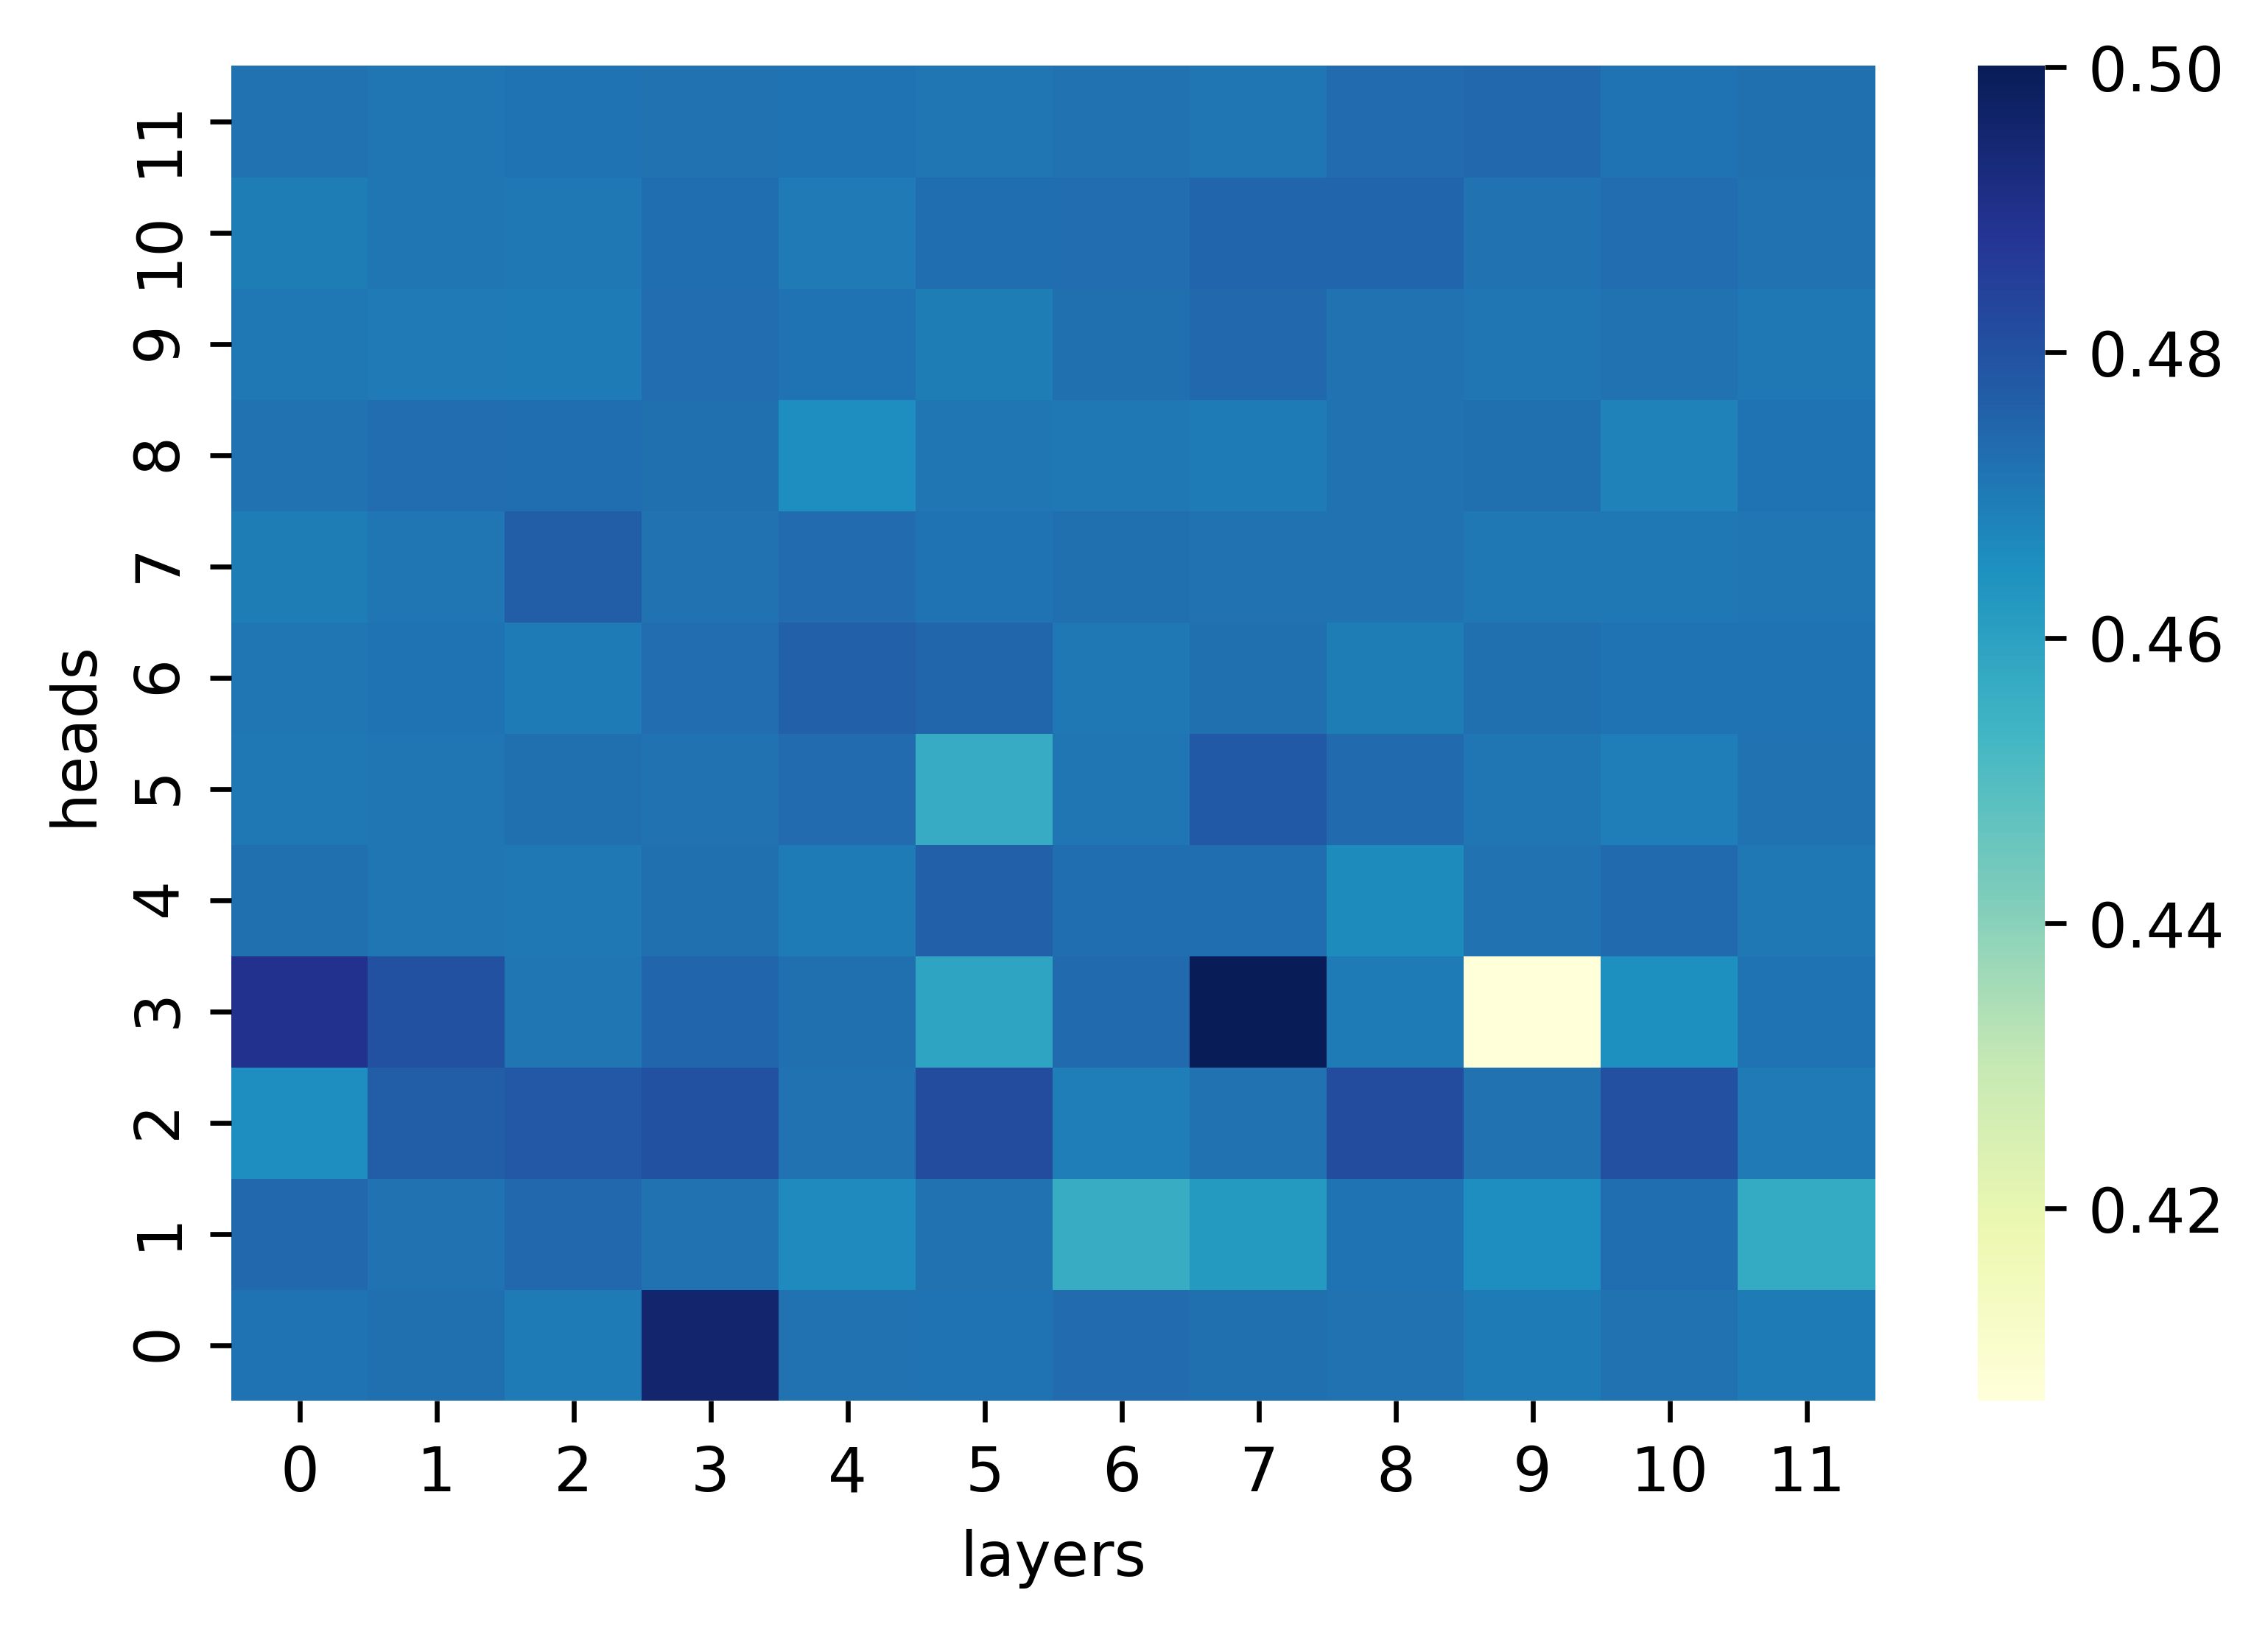
\includegraphics[width=0.75\linewidth]{heads}
			\figlabel{fig:heads}
		\end{minipage}%
	}%
	\subfigure[layers]{
		\begin{minipage}[r]{0.5\linewidth}
			\centering
			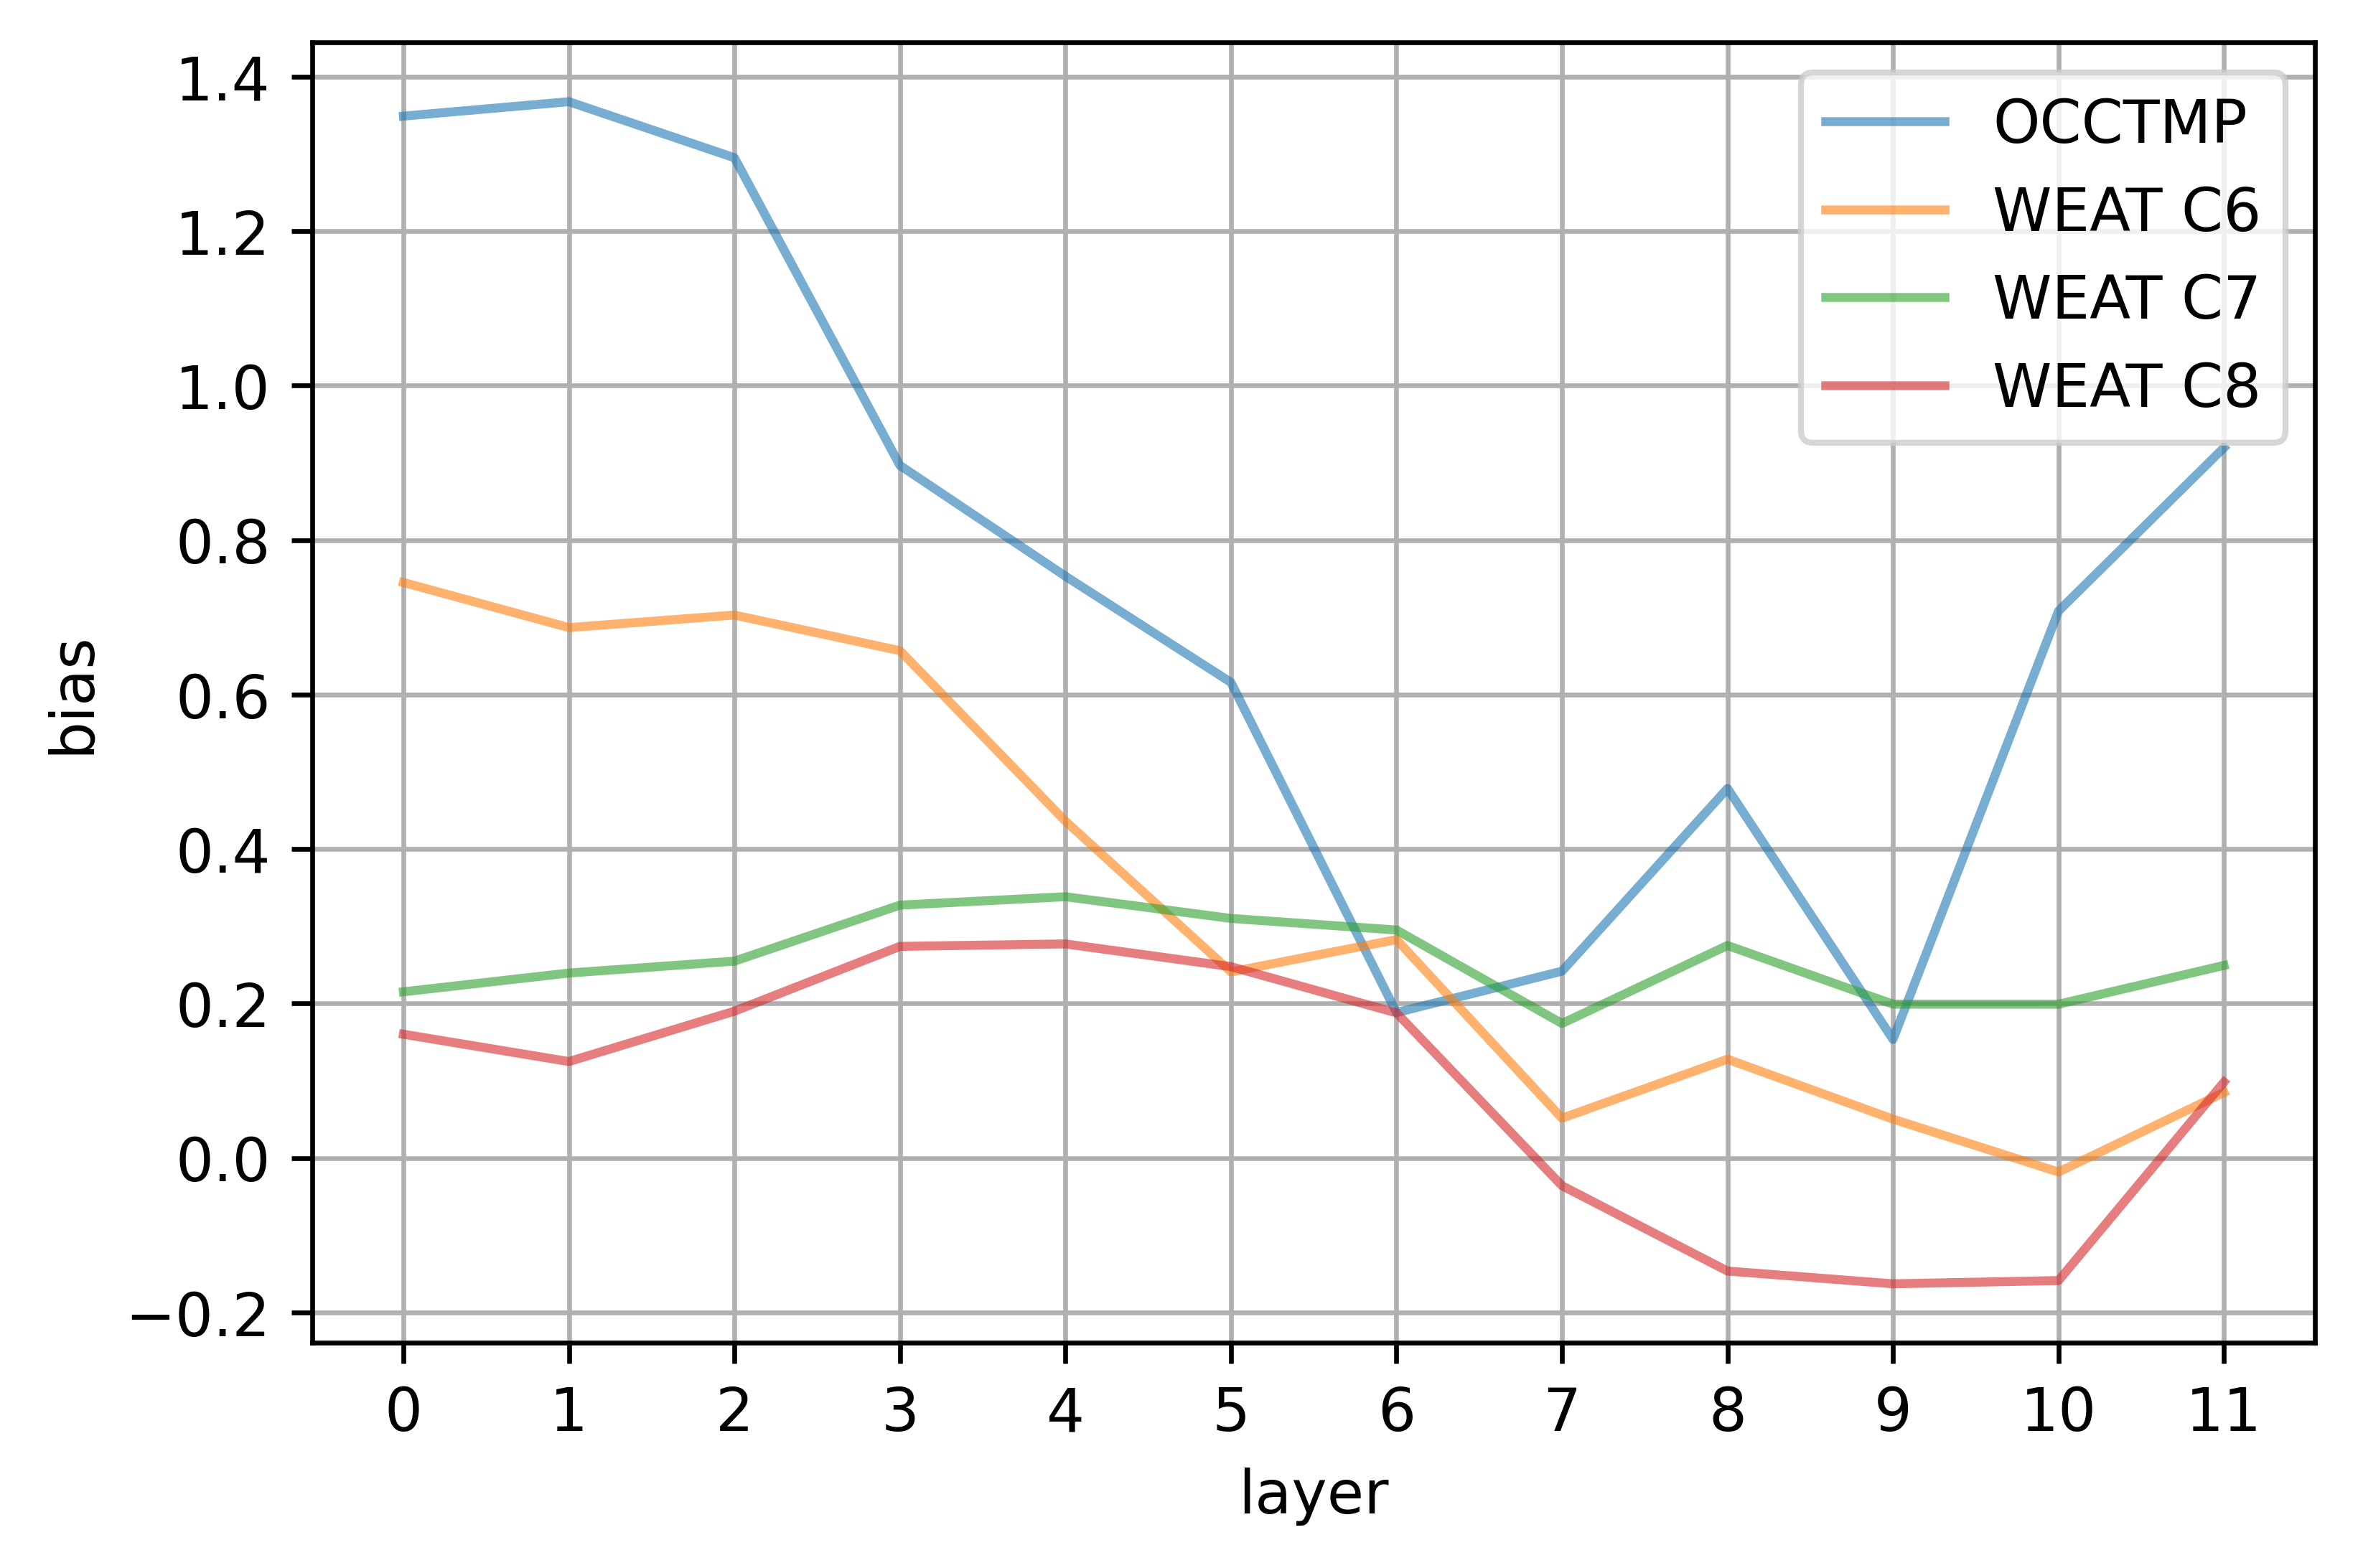
\includegraphics[width=0.75\linewidth]{layers}
			\figlabel{fig:layersbase}
		\end{minipage}%
	}%
	\centering
	\caption{(a): DensRay debiasing on each single attention head in bert-base, measured by \text{diff} on OCCTMP. (b): DensRay debiasing on each single layer, measured by \text{diff} on  OCCTMP and $d$-value on WEAT.}
	\figlabel{fig:headsandlayers}
\end{figure}

\subsubsection*{Quantifying Gender Bias with DensRay}
\seclabel{quantify}
DensRay can be used to quantify gender bias for sentences
and tokens. We use the distance to the origin in the gender
subspace as the measurement. In BERT, we use the average
bias score of tokens to quantify the whole
sentence. \tabref{t:measure1} compares DensRay with the log
probability score \cite{kurita2019measuring}, which
quantifies gender bias based on templates of form ``[TARGET]
is a [ATTRIBUTE]''. We regard zero as a balance point
without bias. Contrary to the log probability score, a
positive DensRay score represents the level of female
bias. These examples show that DensRay is more versatile, it
can quantify  bias both on the token and on the sentence level in contrast to the log-probability score.
In the sentence ``The professor asked the nurse .'' one can immediately see that the model has a male bias on ``professor'' and a female bias on ``nurse'', although the sentence itsel
is completely gender-neutral.

\begin{table}[h]
	\centering
	\scriptsize
	\begin{tabular}{cccccc|c||c}
		\hline
		\multicolumn{6}{c|}{DensRay}&Avg.&log probability score\\		
		\hline\hline
		[MASK] &is &a &professor& . &&&\\
		-0.69 &-0.97 &-0.9  &-0.15  &0.45& &-0.45& 0.63\\
		\hline
		[MASK] &is &a &nurse& . &&&\\
		2.43  &1.34  &1.7   &1.93  &0.5&& 1.58 &-5.44\\
		\hline
		The &professor &asked &me& . &&&\\
		-1.25 &-0.55 &-0.08  &0.59  &0.35 &&-0.19 &
                not applicable\\
		\hline
		The &professor &asked &the&nurse &.&&\\
		-1.3&  -0.25  &0.24  &1.28  &2.19
                &0.45&0.43& not applicable\\
		\hline
	\end{tabular}
	\caption{\tablabel{t:measure1}
		Examples for quantifying bias (model: bert-base).}
\end{table}



\subsubsection*{Number of Training Samples}
In the experiments, we collected training samples for DensRay by considering occurrences of the same word in the corpus across different sentences. This greatly enriches training samples. We also collected equally many masculine and feminine words for data balancing. Now we analyze the impact of these processes. DensRay is essentially a supervised learning method. It is difficult to extract useful features in the case of insufficient or unbalanced labels.  As shown in \figref{curve}, the debiasing results improve with an increased number of training samples.

As a projection-based debiasing method, the premise of DensRay debiasing is that the gender direction should be correct. Unbalanced samples will lead to incorrect gender direction biased towards either the male or the female, resulting in reversing the gender bias during debiasing. For example, if there are more masculine samples, then the embeddings will be biased towards feminine after debiasing. 
%Besides, \eqref{eq:densray3} shows that .
 The figure also shows that a balanced training set improves  debiasing performance.
\begin{figure}[h]
	\centering
	\footnotesize
	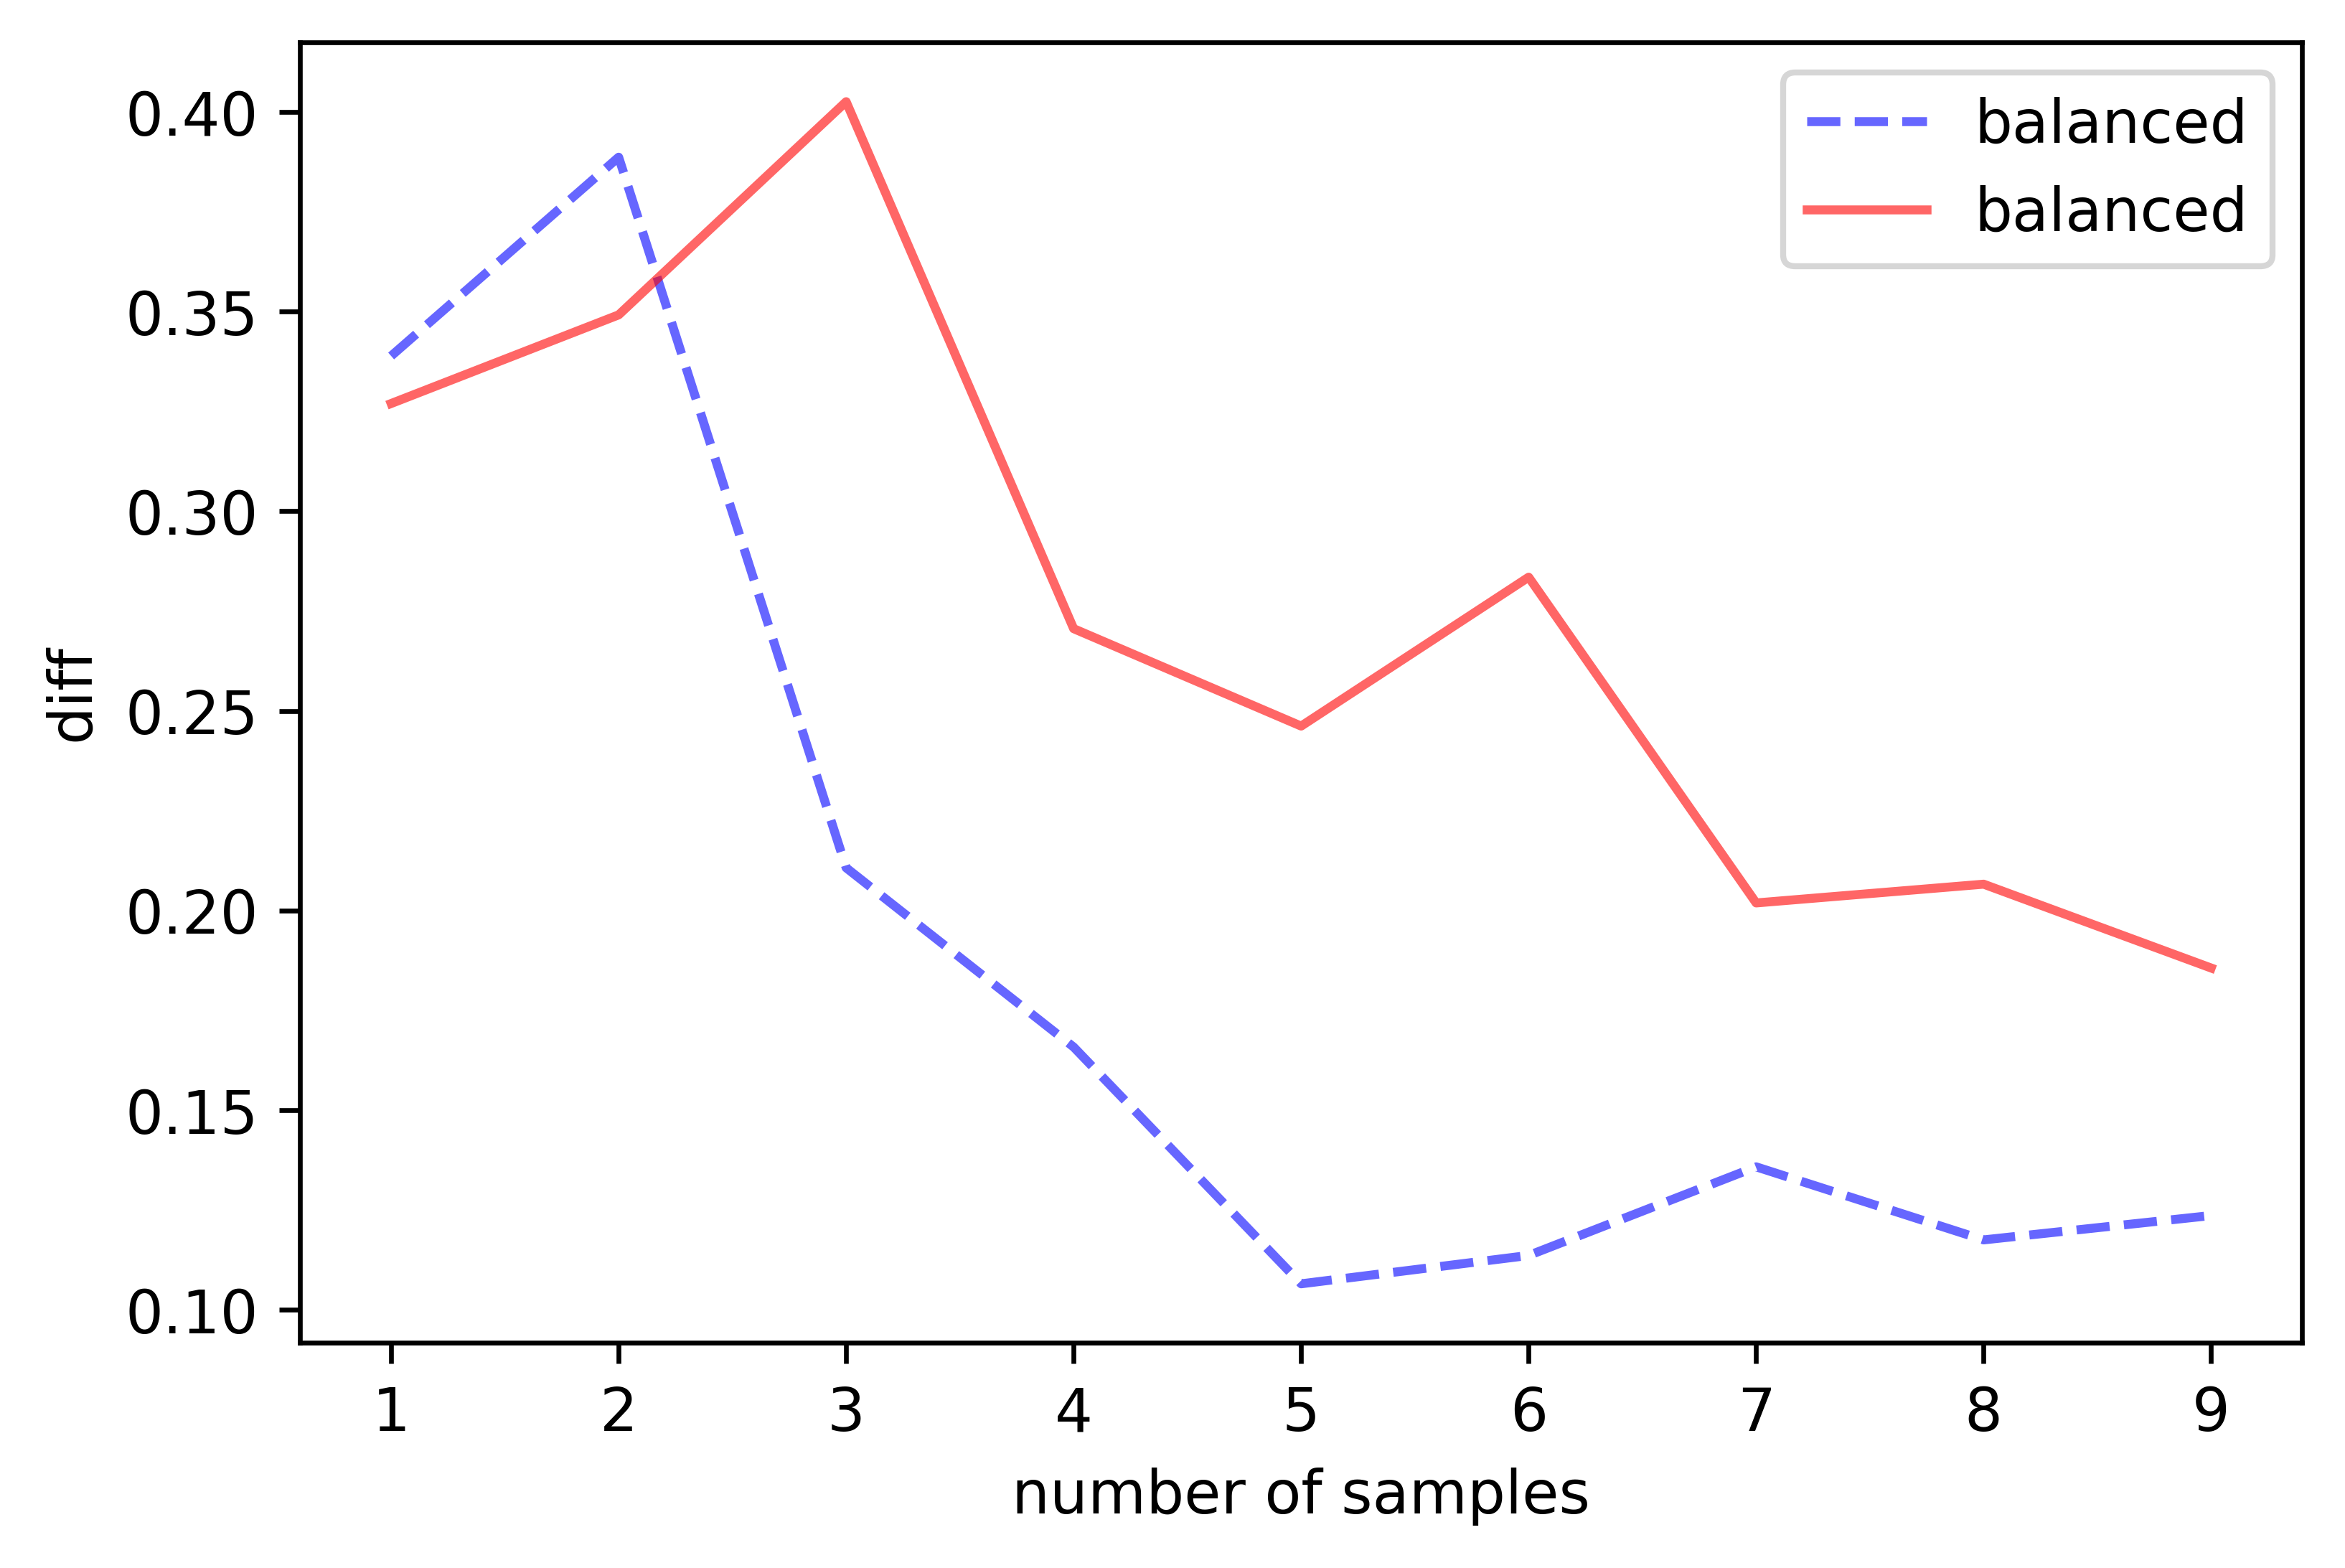
\includegraphics[width=0.4\linewidth]{samples}
	\caption{DensRay debiasing results on OCCTMP with different number of samples and unbalanced/balanced data.}
	\figlabel{curve}
\end{figure}


\subsubsection*{Alternatives to Removing the Gender Dimension}
In our experiments, we zero out the dimensions of the gender
subspace to remove gender bias. 
We also explored three alternatives to zeroing out. 1)
Replace the first dimension of the gender subspace with the
mean value of the first dimension of the training
samples. 2) Standardize the first dimension. 3) Replace the
first dimension with a small random variable sampled from a Gaussian distribution. All of them did not perform well. We further checked the mean and found that the mean of the different layers is not stable around zero, which we plan to investigate in future work. Using higher dimensional gender subspaces (i.e., not only a single direction)
did not improve the debiasing results while harming the model performance.


\subsection{Multilingual Debiasing}
We now show that, in a multilingual contextualized language model like mBERT, we can use DensRay for zero-shot debiasing. Specifically, we train a DensRay model on English and use it to debias Chinese.
We use  bert-base-multilingual-uncased from
\cite{wolf2019huggingfaces}. We use the same setup as for
bert-base-uncased in our previous experiments. As before, we
compute the rotation matrices using the English gendered
words from the ``family'' category of the Google analogy
test set \cite{mikolov2013efficient}.

Since Chinese is a language that does not mark gender, we can construct the OCCTMP templates by directly translating from the English templates. We use the following form:
``\text{[MASK]}\yin{是一个}\textit{occupation}\yin{。}'' We translate the occupation using Tencent Translation\footnote{https://fanyi.qq.com/} and make some manual adjustments to the translation. After removing duplicates,  302 Chinese templates remain.

\tabref{t:templates3} gives results for the Chinese templates. Two examples are given in \tabref{t:templates3}. We see that DensRay trained with English can mitigate gender bias in mBERT: the diff score drops from 1.39 to 1.22 on Chinese templates. 
\begin{table}[h]
	\centering
	\footnotesize
	\begin{tabular}{lccccc}
		\hline
		model & prob(he) & prob(she) & sum &diff & var\\
		\hline
		 bert-multi-en 
		& 0.51 & 0.14 & 0.65 & 1.66&0.81 \\ 
		bert-multi-densray-en & 0.33 & 0.12 & 0.46 & 1.33&0.65 \\
		\hline
		 bert-multi-cn 
		& 0.24 & 0.07 & 0.31 & 1.39&0.60 \\
		 bert-multi-densray-cn 
		& 0.12 & 0.04 & 0.17 & 1.22&0.47\\
		\hline
	\end{tabular}
	\caption{\tablabel{t:templates3}
		Results of OCCTMP on mBERT after applied DensRay. Models with \textit{-en} are tested on English templates, and those with \textit{-cn} are tested on Chinese templates.}
\end{table}

\begin{table}[h]
	\centering
	\footnotesize
	\begin{tabular}{llcccc}
		\hline
		sentence & model & \yin{prob(他)} & \yin{prob(她)}&sum&diff\\
		\hline
		\yin{\text{[MASK]}是一个客座教授。} & bert-multi-en & 0.68 & 0.16&0.84&1.45\\
		\text{[MASK]} is an adjunct professor.& bert-multi-densray-en & 0.51 & 0.18&0.70&1.04\\
		& bert-multi-cn & 0.52 & 0.11&0.63&1.55\\
		& bert-multi-densray-cn & 0.30 & 0.08&0.38&1.31\\
		\hline
		\yin{\text{[MASK]}是一个管理员。} & bert-multi-en & 0.53 & 0.17&0.70&1.14\\
		\text{[MASK]}is an administrator.& bert-multi-densray-en & 0.35 & 0.13&0.48&0.99\\
		& bert-multi-cn & 0.68 & 0.16&0.84&1.45\\
		& bert-multi-densray-cn & 0.51 & 0.18&0.69&1.04\\
		\hline
	\end{tabular}
	\caption{\label{t:templates3}
		Sanity check on the Chinese templates, where \yin{\textit{他}} means \textit{he} and \yin{\textit{她}} means \textit{she}. Corresponding English translations are shown below the Chinese.}
\end{table}


%\section{DensRay Debiasing multilingual-BERT}
%\subsection{Setup}
As an extension, we apply DensRay to mBERT for zero-shot debiasing on Chinese. Here we use the "bert-multilingual-uncesed" model from \citep{wolf2019huggingfaces}, we also use the same setup as the "bert-base-uncased" model in our previous experiments. 

Still, we compute the rotation matrices by the English gendered words from the "family" category of the Google analogy test set \citep{mikolov2013efficient}.

Since Chinese is a language that doesn't contain genus, we can construct the templates by simply translating from the English templates. After removing the duplicates, we get 302 Chinese templates.

\subsection{Results on Templates}
Results about our experiments on the templates are summarized in table \ref{t:templates2}. Two example templates are given in table \ref{t:templates2}. The evaluation on our templates shows that DensRay can mitigate the gender bias on BERT.
\begin{table*}[ht]
\centering
\begin{tabular}{lllll}
\hline
model & prob(he) & prob(she) & diff & var\\
\hline
bert-multi-en & 0.5064 & 0.1427 & 0.3637 & 0.0619 \\
bert-multi-densray-en & 0.3344 & 0.1207 & 0.2137 & 0.0277 \\
bert-multi-cn & 0.2370 & 0.0718 & 0.1652 & 0.0223 \\
bert-multi-densray-cn & 0.1247 & 0.0407 & 0.0840 & 0.0055\\
\hline
\end{tabular}
\caption{\label{t:templates2}
Results of templates on mBERT after applied DensRay. Models with \textit{-en} are tested on our English templates, and those with \textit{-cn} are tested on our Chinese templates.}
\end{table*}

\begin{table}[ht]
\centering
\begin{tabular}{llll}
\hline
model & ppl\\
\hline
bert-multi & 3.5788\\
bert-multi-densray & 3.7216\\
\hline
\end{tabular}
\caption{\label{t:ppl2}
Language modeling performance on mBERT after applied DensRay.}
\end{table}

We also checked the perplexity for mBERT on Wikitext-2, see table \ref{t:ppl2}. Results show that DensRay can be extended to mBERT as a zero-shot debiasing method for some other languages.

\begin{table*}[t]
\centering
\begin{tabular}{llll}
\hline
sentence & model & prob(he) & prob(she)\\
\hline
[MASK] is a adjunct professor. & bert-multi-en & 0.6823 & 0.1611\\
 & bert-multi-densray-en & 0.5073 & 0.1762\\
& bert-multi-cn & 0.5189 & 0.1108\\
 & bert-multi-densray-cn & 0.3046 & 0.0831\\
\hline
[MASK] is a administrator. & bert-multi-en & 0.5344 & 0.1670\\
 & bert-multi-densray-en & 0.3496 & 0.1318\\
& bert-multi-cn & 0.6823 & 0.1611\\
 & bert-multi-densray-cn & 0.5073 & 0.1762\\
\hline
\end{tabular}
\caption{\label{t:templates3}
Sanity check on the Chinese templates. Here we only present their translation for convenience.}
\end{table*}

\section{Related Work}
\subsection{Quantifying Gender Bias}
\textbf{Association tests} are commonly used to measure
gender bias. The original WEAT is used on static
embeddings. To extend WEAT to contextual embeddings, some
template-based processes
\cite{karve2019conceptor,kurita2019measuring,Tan2019AssessingSA}
were constructed to obtain the word embeddings from the
context. SEAT further improved the templates and computed
the similarities between the sentences instead of
words. \newcite{guo2020detecting} proposed CEAT (Contextual
Embedding Association Test), which samples the occurrences
from the corpus to get the embeddings, and measures the bias
by a random-effects model. However, we find that it is
difficult to obtain a stable result on CEAT due to the
\enote{hs}{what does vary mean?} vary
contexts, so in this paper we  use WEAT and SEAT for our
experiments. \newcite{kurita2019measuring} proposed a
template-based log probability bias score to measure the
association between targets and attributes in BERT. Since it
can only be applied on specific templates, we compare this
method with DensRay as a measurement of gender bias in
\secref{quantify}.

An alternative way to measure gender bias is to evaluate on
\textbf{downstream tasks}. For coreference resolution,
\newcite{zhao2018gender} designed Winobias and
\newcite{rudinger2018gender} designed Winogender
schemas. \newcite{webster2018mind} released GAP, a balanced
corpus of Gendered Ambiguous Pronouns, which measures gender
bias as the ratio of F1 score on masculine to F1 score on
feminine. However the ratio is very close to 1
\cite{Chada_2019,Attree_2019} making it hard to compare
debiasing systems. For sentiment analysis, Equity Evaluation
Corpus (EEC) \cite{Kiritchenko_2018} was designed to measure
gender bias by the difference in emotional intensity
predictions between gender-swapped sentences. Since the
measurements of gender bias in these data sets are not
intuitive, we chose to use association tests in
this paper.

\subsection{Debiasing Methods}
Many methods to remove gender bias have been proposed. The most common way is to define a gender direction (or, more generally, a subspace) by a set of gendered words and debias the word embeddings in a post-processing projection. \cite{bolukbasi2016man} propose (i) \emph{hard debiasing}: use the gendered words to compute the difference embedding vector as the gender direction; and (ii) \emph{soft debiasing}, a machine learning based method that combines the inner-products objective of word embedding and an objective to project the word embedding into an orthogonal gender subspace. It has been found to work better than soft debiasing.  \cite{dev2019attenuating} explored partial projection and some simple tricks to improve the hard debiasing method. \cite{zhao2019gender} applied the data augmentation and debiasing method of  \cite{bolukbasi2016man} to mitigate gender bias on ELMo  \cite{Peters:2018}. \cite{karve2019conceptor} proposed the debiasing conceptor, which shrinks each principal component of the covariance matrix of the embeddings to achieve a soft debiasing. They also introduced a simple and intuitive hard debiasing method proposed by \cite{mu2018all}, which identified the gender subspace by PCA and projected the first principal component off.  

The debiasing conceptor and the \cite{mu2018all} hard debiasing produce gender direction by gendered word list mixed with male and female words. In contrast, the \cite{bolukbasi2016man} hard debiasing used two groups of gendered words for definition and another two groups for alignment, to identify the gender direction by male-female pairs. The method we use, DensRay, is similar to the \cite{bolukbasi2016man} hard debiasing in this aspect. However, DensRay uses only one male and one female word list, and it can be solved efficiently in a closed form. So it would be more stable to be applied to contextual models than the \cite{bolukbasi2016man} hard debiasing. 
 





\section{Conclusion}
We introduced DensRay debiasing on BERT. Our experiments
showed that this method can effectively mitigate gender bias on OCCTMP and the Association Tests, while maintained the performance of BERT on language modeling and GLUE tasks. We applied DensRay to BERT attention heads, showed that gender information is processed in all attention heads, there is no single attention head responsible for processing gender information. We also used DensRay to obtain interpretable gender bias scores, to quantify bias on token and sentence level for all representations. Finally, we demonstrated that we can remove bias multilingually, we used only English training data to effectively debias Chinese.



%\section*{Acknowledgements}

%The acknowledgements should go immediately before the references.  Do
%not number the acknowledgements section. Do not include this section
%when submitting your paper for review.

% include your own bib file like this:
\bibliographystyle{coling}
\bibliography{coling2020}

%\begin{thebibliography}{}

%\bibitem[\protect\citename{Aho and Ullman}1972]{Aho:72}
%Alfred~V. Aho and Jeffrey~D. Ullman.
%\newblock 1972.
%\newblock {\em The Theory of Parsing, Translation and Compiling}, volume~1.
%\newblock Prentice-{Hall}, Englewood Cliffs, NJ.

%\bibitem[\protect\citename{{American Psychological Association}}1983]{APA:83}
%{American Psychological Association}.
%\newblock 1983.
%\newblock {\em Publications Manual}.
%\newblock American Psychological Association, Washington, DC.

%\bibitem[\protect\citename{{Association for Computing Machinery}}1983]{ACM:83}
%{Association for Computing Machinery}.
%\newblock 1983.
%\newblock {\em Computing Reviews}, 24(11):503--512.

%\bibitem[\protect\citename{Chandra \bgroup et al.\egroup }1981]{Chandra:81}
%Ashok~K. Chandra, Dexter~C. Kozen, and Larry~J. Stockmeyer.
%\newblock 1981.
%\newblock Alternation.
%\newblock {\em Journal of the Association for Computing Machinery},
%  28(1):114--133.

%\bibitem[\protect\citename{Gusfield}1997]{Gusfield:97}
%Dan Gusfield.
%\newblock 1997.
%\newblock {\em Algorithms on Strings, Trees and Sequences}.
%\newblock Cambridge University Press, Cambridge, UK.

%\bibitem[\protect\citename{Rasooli and Tetreault}2015]{rasooli-tetrault-2015}
%Mohammad~Sadegh Rasooli and Joel~R. Tetreault. 2015.
%\newblock {Yara parser: {A} fast and accurate dependency parser}.
%\newblock \emph{Computing Research Repository}, arXiv:1503.06733.
%\newblock Version 2.

%\bibitem[\protect\citename{Borschinger and Johnson}2011]{borsch2011}
%Benjamin Borschinger and Mark Johnson. 2011.
%\newblock A particle filter algorithm for {B}ayesian wordsegmentation.
%\newblock In \emph{Proceedings of the Australasian Language Technology Association %Workshop 2011}, pages 10--18, Canberra, Australia.

%\end{thebibliography}

\end{document}
